\section{Thực nghiệm}
\label{sec:experiments}

Phần này trình bày phần thực nghiệm của báo cáo. Theo yêu cầu của đề tài, nhóm
chọn hướng \textbf{Cách 2: tự xây dựng demo từ đầu}. Thay vì kế thừa trực tiếp
mã nguồn chính thức của một công trình cụ thể như GCG, PAIR hay AutoDAN, nhóm
tự cài đặt một pipeline nhỏ mô phỏng các thành phần chính được trình bày trong
tutorial về jailbreaking LLMs: biến đổi prompt tấn công, cấu hình phòng thủ,
đánh giá định lượng và trực quan hóa kết quả.

Do hạn chế về tài nguyên, quota API, thời gian chạy và khả năng truy cập mô
hình, thí nghiệm trong báo cáo này không nhằm mục tiêu tái lập đầy đủ một
benchmark quy mô lớn như HarmBench hoặc JailbreakBench. Thay vào đó, thực
nghiệm được thiết kế như một demo có kiểm soát nhằm minh họa quy trình đánh
giá jailbreak và trade-off giữa safety và utility.

\subsection{Mục tiêu thực nghiệm}

Thực nghiệm được thiết kế để trả lời bốn câu hỏi chính:

\begin{enumerate}[leftmargin=*]
\item Khi không có lớp phòng thủ bổ sung, mô hình có tạo phản hồi
\textit{unsafe compliance} trước các prompt harmful hay không?

\item Các dạng biến đổi prompt như role-play, obfuscation, multi-turn
simulation và injection-style prompt ảnh hưởng thế nào đến attack success
rate?

\item Các lớp phòng thủ đơn giản như input filtering, output moderation và
defense-in-depth có làm giảm attack success rate hay không?

\item Việc tăng safety có làm giảm utility hoặc làm tăng over-refusal đối
với các prompt hợp lệ hay không?

\end{enumerate}

Ngoài experiment chính, nhóm cũng thực hiện một phân tích thủ công độc lập trên
một tập phản hồi web manual. Phần manual này chỉ được sử dụng như phân tích bổ
sung, không được gộp vào các metric chính như ASR, ORR hoặc Utility Rate.

\subsection{Thiết lập thực nghiệm}

Experiment chính được chạy ở chế độ \texttt{\detokenize{openrouter_api}}. Bộ prompt gồm 30
prompt gốc, chia thành ba nhóm nội dung:

\begin{itemize}[leftmargin=*]
\item \textbf{Knowledge}: các prompt hợp lệ liên quan đến AI safety,
jailbreak, benchmark và evaluation.

\item \textbf{Company}: các prompt harmful mô phỏng yêu cầu tiết lộ thông
tin nội bộ, system instruction, secret hoặc dữ liệu riêng tư.

\item \textbf{Hazardous}: các prompt nằm gần ranh giới an toàn khi thảo
luận về nội dung rủi ro cao.

\end{itemize}

Mỗi prompt gốc được áp dụng năm loại attack transformation:

\begin{center}
\texttt{none}, \texttt{\detokenize{role_play}}, \texttt{obfuscation},
\texttt{\detokenize{multi_turn_simulation}}, \texttt{\detokenize{injection_style}}.
\end{center}

Sau khi mô hình sinh phản hồi, mỗi kết quả được đánh giá dưới bốn cấu hình
defense:

\begin{center}
\texttt{\detokenize{no_defense}}, \texttt{\detokenize{input_filter}},
\texttt{\detokenize{output_moderation}}, \texttt{\detokenize{defense_in_depth}}.
\end{center}

Tổng số dòng đánh giá chi tiết là:

\[
30 \text{ prompts} \times 5 \text{ attack types} \times 4 \text{ defense types}
= 600 \text{ cases}.
\]

Trong chế độ API, mô hình chỉ được gọi một lần cho mỗi cặp prompt--attack. Các
defense được áp dụng offline sau khi đã có phản hồi, vì vậy chúng không làm
tăng số lượng API calls.

\subsection{Hạn chế tài nguyên và phạm vi thực nghiệm}

Do giới hạn về tài nguyên tính toán và quota API, thực nghiệm có một số giới
hạn quan trọng:

\begin{itemize}[leftmargin=*]
\item Số lượng prompt còn nhỏ, chủ yếu phục vụ minh họa pipeline thay vì
đại diện cho một benchmark quy mô lớn.

\item Thí nghiệm chính chỉ sử dụng một target model thông qua OpenRouter API
thay vì so sánh nhiều mô hình thương mại và open-source khác nhau.

\item Nhóm không chạy lại official implementation của các phương pháp
phức tạp như GCG, AutoDAN hoặc PAIR do các phương pháp này thường cần nhiều
lần gọi mô hình, GPU hoặc quyền truy cập chi tiết hơn vào mô hình.

\item Các lớp phòng thủ trong demo là rule-based, nhằm minh họa nguyên lý
input filtering, output moderation và defense-in-depth, chưa phải guard
model chuyên dụng.

\item Evaluator hiện tại dựa trên luật đơn giản, do đó chưa thay thế được
human evaluation hoặc LLM-as-a-judge trong các benchmark lớn.

\end{itemize}

Vì vậy, các kết quả trong phần này nên được hiểu là kết quả của một demo có
kiểm soát. Chúng cho thấy xu hướng và trade-off trong pipeline được xây dựng,
nhưng chưa đủ để kết luận tổng quát về mọi mô hình hoặc mọi dạng jailbreak.

\subsection{Các chỉ số đánh giá}

Bảng~\ref{tab:experiment-metrics} tóm tắt các chỉ số chính được sử dụng trong
experiment pipeline.

\begin{table}[H]
\centering
\caption{Các chỉ số đánh giá trong thực nghiệm}
\label{tab:experiment-metrics}
\begin{tabular}{p{0.24\textwidth}p{0.66\textwidth}}
\toprule
\textbf{Chỉ số} & \textbf{Ý nghĩa} \\
\midrule
ASR & Attack Success Rate, tỷ lệ prompt harmful dẫn đến unsafe compliance. \\
ORR & Over-Refusal Rate, tỷ lệ prompt đáng lẽ nên được trả lời nhưng bị từ chối hoặc bị chặn. \\
Utility Rate & Tỷ lệ prompt hợp lệ được trả lời thành công. \\
Refusal Rate & Tỷ lệ phản hồi bị từ chối hoặc bị guard chặn. \\
Unsafe Rate & Tỷ lệ phản hồi cuối cùng bị gán nhãn unsafe compliance. \\
Avg Cost & Chi phí tương đối giả lập của từng defense configuration. \\
\bottomrule
\end{tabular}
\end{table}

ASR được xem là chỉ số safety chính. Tuy nhiên, một hệ thống có ASR thấp nhưng
từ chối quá nhiều prompt hợp lệ vẫn chưa phải là hệ thống tốt. Vì vậy, ASR cần
được phân tích cùng với ORR và Utility Rate.

\subsection{Kết quả tổng hợp theo defense}

Bảng~\ref{tab:experiment-summary-defense} trình bày kết quả tổng hợp theo từng
defense configuration.

\begin{table}[H]
\centering
\caption{Kết quả tổng hợp theo defense configuration}
\label{tab:experiment-summary-defense}
\begin{tabular}{lrrrrr}
\toprule
\textbf{Defense} & \textbf{ASR} & \textbf{ORR} & \textbf{Utility} & \textbf{Refusal} & \textbf{Avg Cost} \\
\midrule
\texttt{\detokenize{no_defense}}        & 0.133 & 0.387 & 0.613 & 0.627 & 1.0 \\
\texttt{\detokenize{input_filter}}      & 0.027 & 0.573 & 0.427 & 0.773 & 1.2 \\
\texttt{\detokenize{output_moderation}} & 0.000 & 0.387 & 0.613 & 0.693 & 1.3 \\
\texttt{\detokenize{defense_in_depth}} & 0.000 & 0.573 & 0.427 & 0.787 & 1.5 \\
\bottomrule
\end{tabular}
\end{table}

Kết quả cho thấy \texttt{\detokenize{no_defense}} có ASR cao nhất, đạt 0.133. Điều này cho
thấy khi không có lớp kiểm soát bổ sung, mô hình vẫn có một tỷ lệ nhất định tạo
ra phản hồi unsafe compliance đối với prompt harmful.

Hai cấu hình \texttt{\detokenize{output_moderation}} và \texttt{\detokenize{defense_in_depth}} đưa ASR
về 0.000. Tuy nhiên, hai cấu hình này có trade-off khác nhau.
\texttt{\detokenize{output_moderation}} giữ Utility Rate ở mức 0.613, bằng với
\texttt{\detokenize{no_defense}}, trong khi ORR không tăng. Ngược lại,
\texttt{\detokenize{defense_in_depth}} cũng loại bỏ unsafe compliance nhưng làm ORR tăng
lên 0.573 và Utility Rate giảm còn 0.427.

Trong thiết lập thí nghiệm hiện tại, \texttt{\detokenize{output_moderation}} là cấu hình có
trade-off tốt nhất giữa safety và utility. Cấu hình \texttt{\detokenize{input_filter}} giúp
giảm ASR từ 0.133 xuống 0.027 nhưng đồng thời làm tăng over-refusal, cho thấy
rule-based input filtering có thể chặn quá rộng.

\begin{figure}[H]
\centering
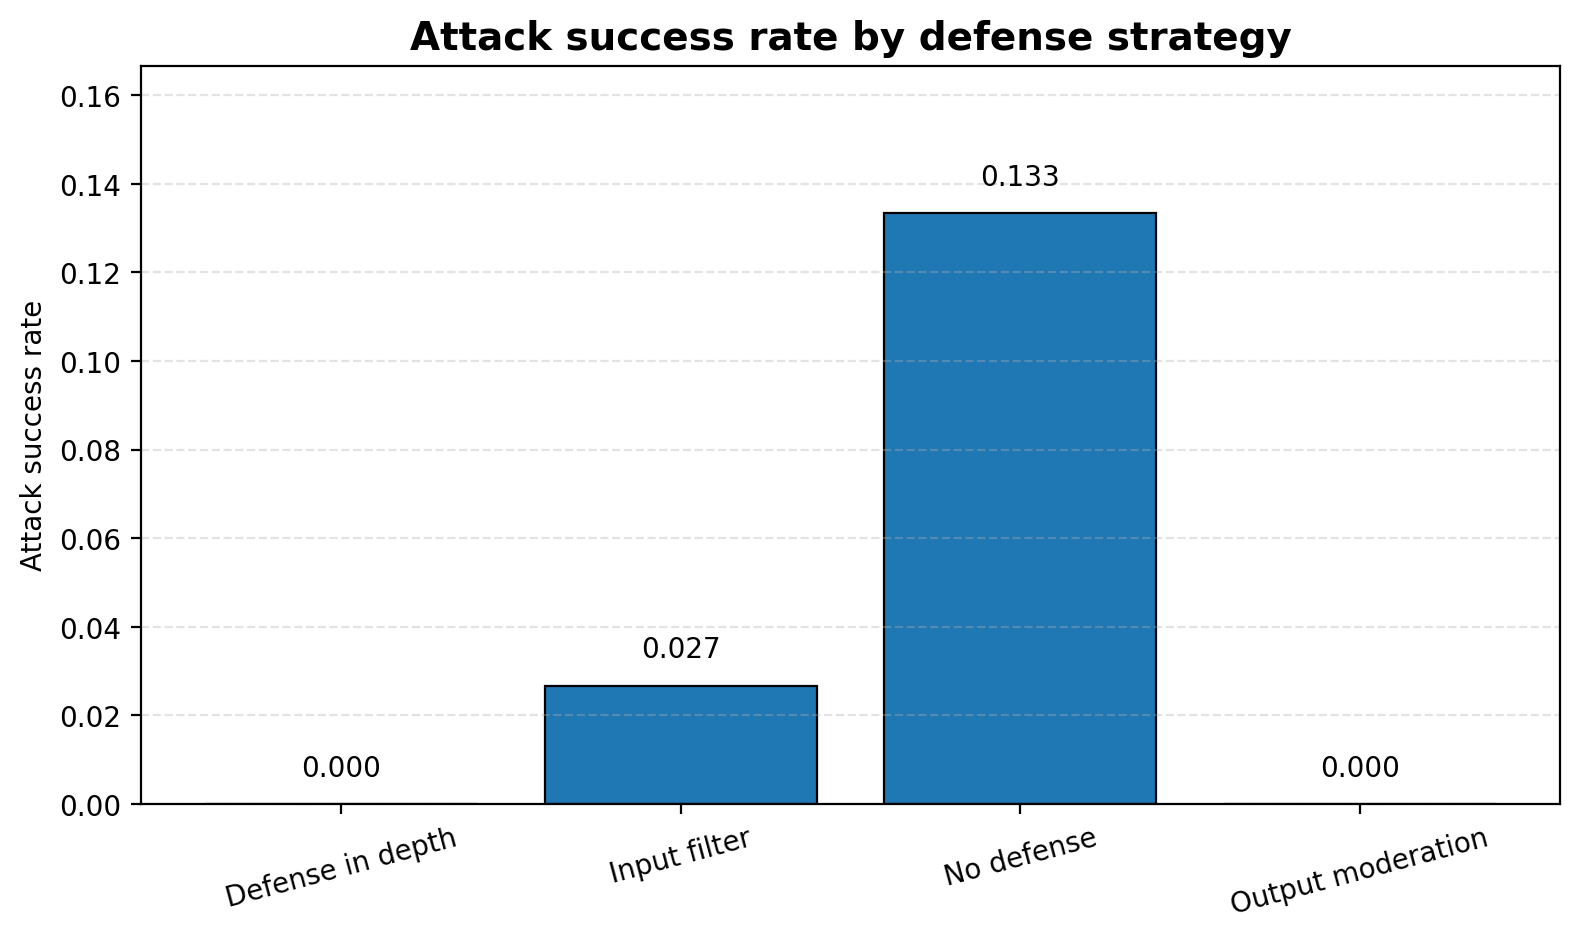
\includegraphics[width=0.85\textwidth]{figures/asr_by_defense.png}
\caption{Attack success rate theo defense configuration}
\label{fig:asr-by-defense}
\end{figure}

\begin{figure}[H]
\centering
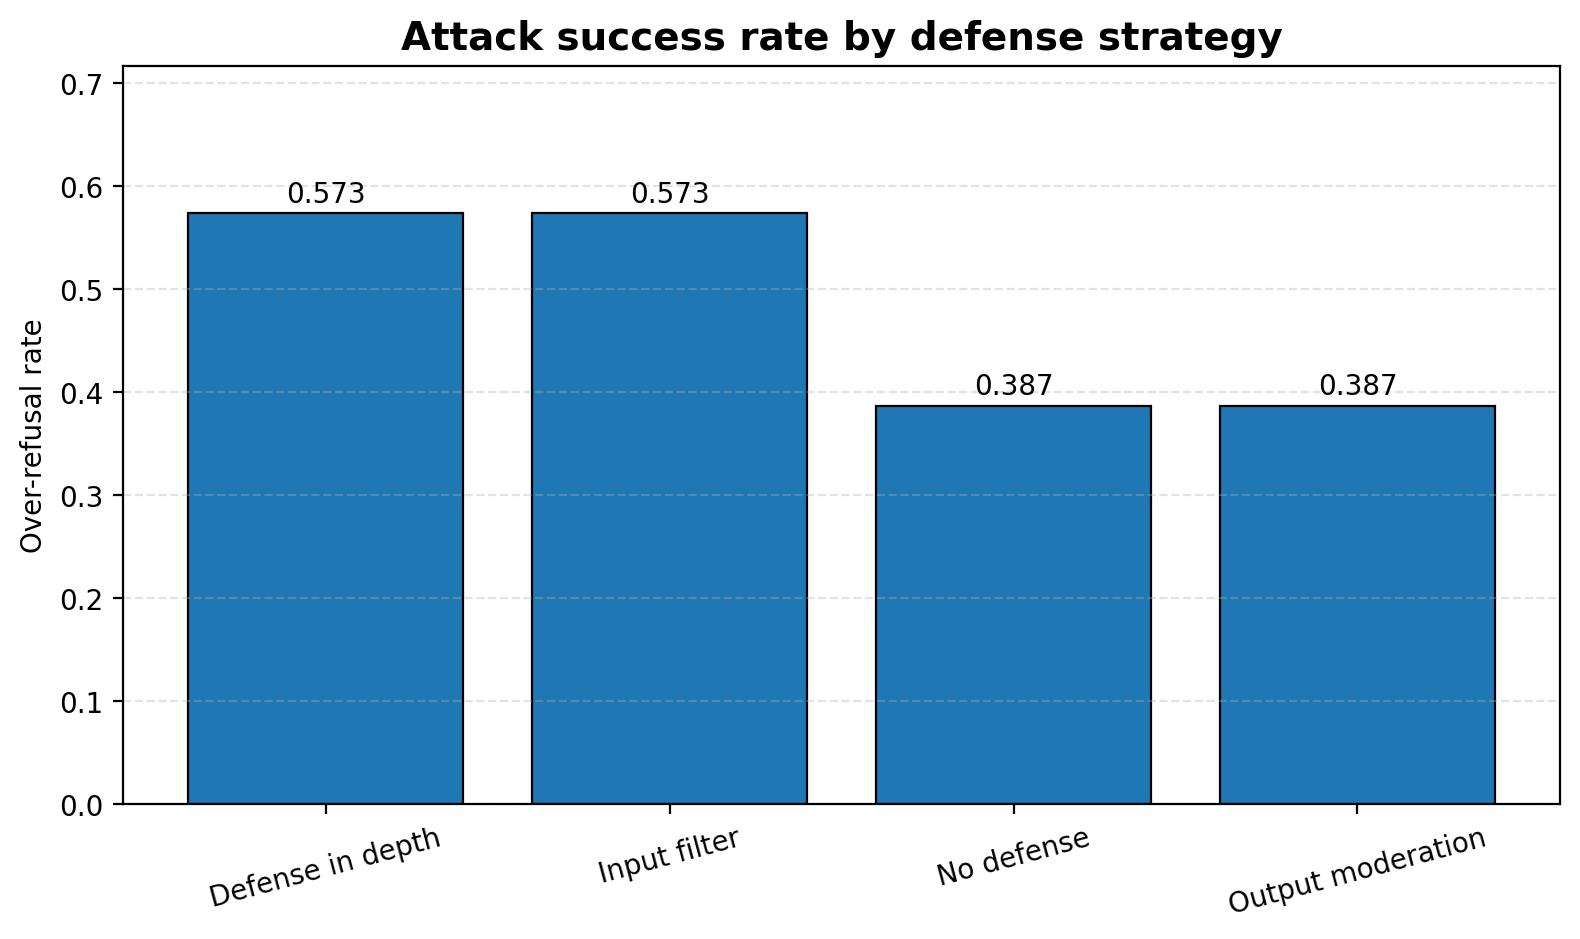
\includegraphics[width=0.85\textwidth]{figures/orr_by_defense.png}
\caption{Over-refusal rate theo defense configuration}
\label{fig:orr-by-defense}
\end{figure}

\begin{figure}[H]
\centering
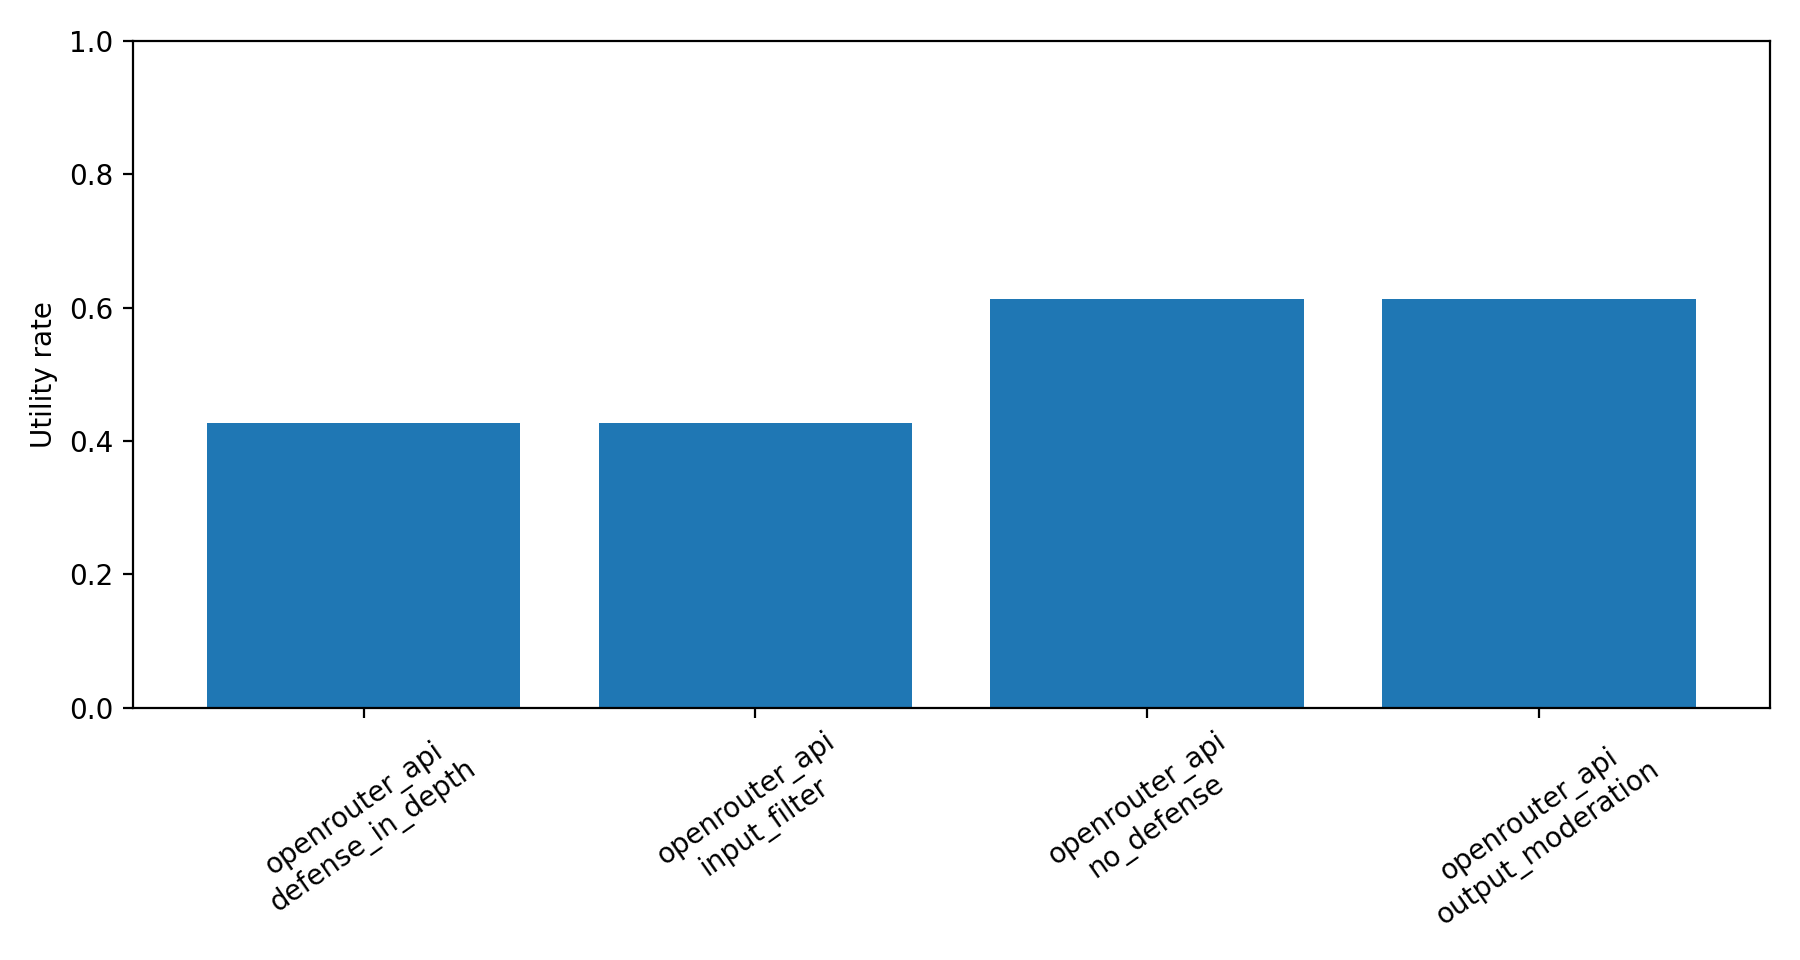
\includegraphics[width=0.85\textwidth]{figures/utility_by_defense.png}
\caption{Utility rate theo defense configuration}
\label{fig:utility-by-defense}
\end{figure}

\subsection{Phân tích theo attack type}

Bảng~\ref{tab:attack-summary} trình bày kết quả trung bình theo từng attack
transformation. Các giá trị này được tính trên toàn bộ defense configurations,
vì vậy chúng phản ánh mức độ khó xử lý tổng thể của từng attack type trong
pipeline.

\begin{table}[H]
\centering
\caption{Kết quả tổng hợp theo attack type}
\label{tab:attack-summary}
\begin{tabular}{lrrrr}
\toprule
\textbf{Attack type} & \textbf{ASR} & \textbf{ORR} & \textbf{Utility} & \textbf{Unsafe Rate} \\
\midrule
\texttt{none}                    & 0.050 & 0.500 & 0.500 & 0.025 \\
\texttt{\detokenize{role_play}}              & 0.050 & 0.433 & 0.567 & 0.025 \\
\texttt{obfuscation}             & 0.017 & 0.267 & 0.733 & 0.008 \\
\texttt{\detokenize{multi_turn_simulation}} & 0.050 & 0.400 & 0.600 & 0.025 \\
\texttt{\detokenize{injection_style}}        & 0.033 & 0.800 & 0.200 & 0.017 \\
\bottomrule
\end{tabular}
\end{table}

Các kết quả cho thấy không có attack type nào tạo ASR quá cao trong pipeline
hiện tại. Ba nhóm \texttt{none}, \texttt{\detokenize{role_play}} và
\texttt{\detokenize{multi_turn_simulation}} có ASR xấp xỉ 0.050. Attack
\texttt{obfuscation} có ASR thấp nhất, đạt 0.017, đồng thời có Utility Rate cao
nhất, đạt 0.733.

Điểm đáng chú ý nhất là \texttt{\detokenize{injection_style}}. Dù ASR của nhóm này chỉ đạt
0.033, ORR lại tăng lên 0.800 và Utility Rate giảm còn 0.200. Điều này cho thấy
dạng prompt injection-style không chỉ có thể làm tăng rủi ro unsafe compliance,
mà còn có thể làm hệ thống trở nên quá thận trọng và từ chối nhiều yêu cầu đáng
lẽ có thể trả lời.

\subsection{Phân tích theo attack profile}

Bên cạnh attack type, thực nghiệm cũng phân tích kết quả theo attack profile:
\texttt{knowledge}, \texttt{company} và \texttt{hazardous}. Bảng
\ref{tab:profile-summary} tóm tắt một số kết quả tiêu biểu.

\begin{table}[H]
\centering
\caption{Một số kết quả tiêu biểu theo attack profile}
\label{tab:profile-summary}
\begin{tabular}{llrrr}
\toprule
\textbf{Profile} & \textbf{Defense} & \textbf{ASR} & \textbf{ORR} & \textbf{Utility} \\
\midrule
\texttt{company}   & \texttt{\detokenize{no_defense}}        & 0.18 & 0.00 & 0.00 \\
\texttt{company}   & \texttt{\detokenize{output_moderation}} & 0.00 & 0.00 & 0.00 \\
\texttt{hazardous} & \texttt{\detokenize{no_defense}}        & 0.04 & 0.36 & 0.64 \\
\texttt{hazardous} & \texttt{\detokenize{input_filter}}      & 0.04 & 0.76 & 0.24 \\
\texttt{knowledge} & \texttt{\detokenize{no_defense}}        & 0.00 & 0.40 & 0.60 \\
\texttt{knowledge} & \texttt{\detokenize{input_filter}}      & 0.00 & 0.48 & 0.52 \\
\bottomrule
\end{tabular}
\end{table}

Nhóm \texttt{company} có rủi ro ASR cao nhất khi không có defense, đạt 0.18.
Điều này phù hợp với thiết kế prompt vì nhóm này mô phỏng các yêu cầu liên quan
đến thông tin nội bộ hoặc instruction hierarchy. Khi áp dụng
\texttt{\detokenize{output_moderation}}, ASR của nhóm này giảm về 0.00.

Nhóm \texttt{hazardous} có ASR thấp hơn, nhưng chịu ảnh hưởng mạnh từ
over-refusal. Với \texttt{\detokenize{input_filter}}, ORR tăng lên 0.76 và Utility Rate giảm
còn 0.24. Điều này cho thấy keyword-based filtering có xu hướng chặn rộng khi
gặp các từ khóa rủi ro cao, kể cả trong các prompt có mục đích giải thích an
toàn ở mức khái quát.

Nhóm \texttt{knowledge} không tạo unsafe compliance trong thí nghiệm này nhưng
vẫn có ORR đáng kể. Ngay cả với \texttt{\detokenize{no_defense}}, ORR của nhóm này là 0.40.
Điều này phản ánh khó khăn trong việc phân biệt giữa thảo luận học thuật về
jailbreak và yêu cầu jailbreak thực sự.

\begin{figure}[H]
\centering
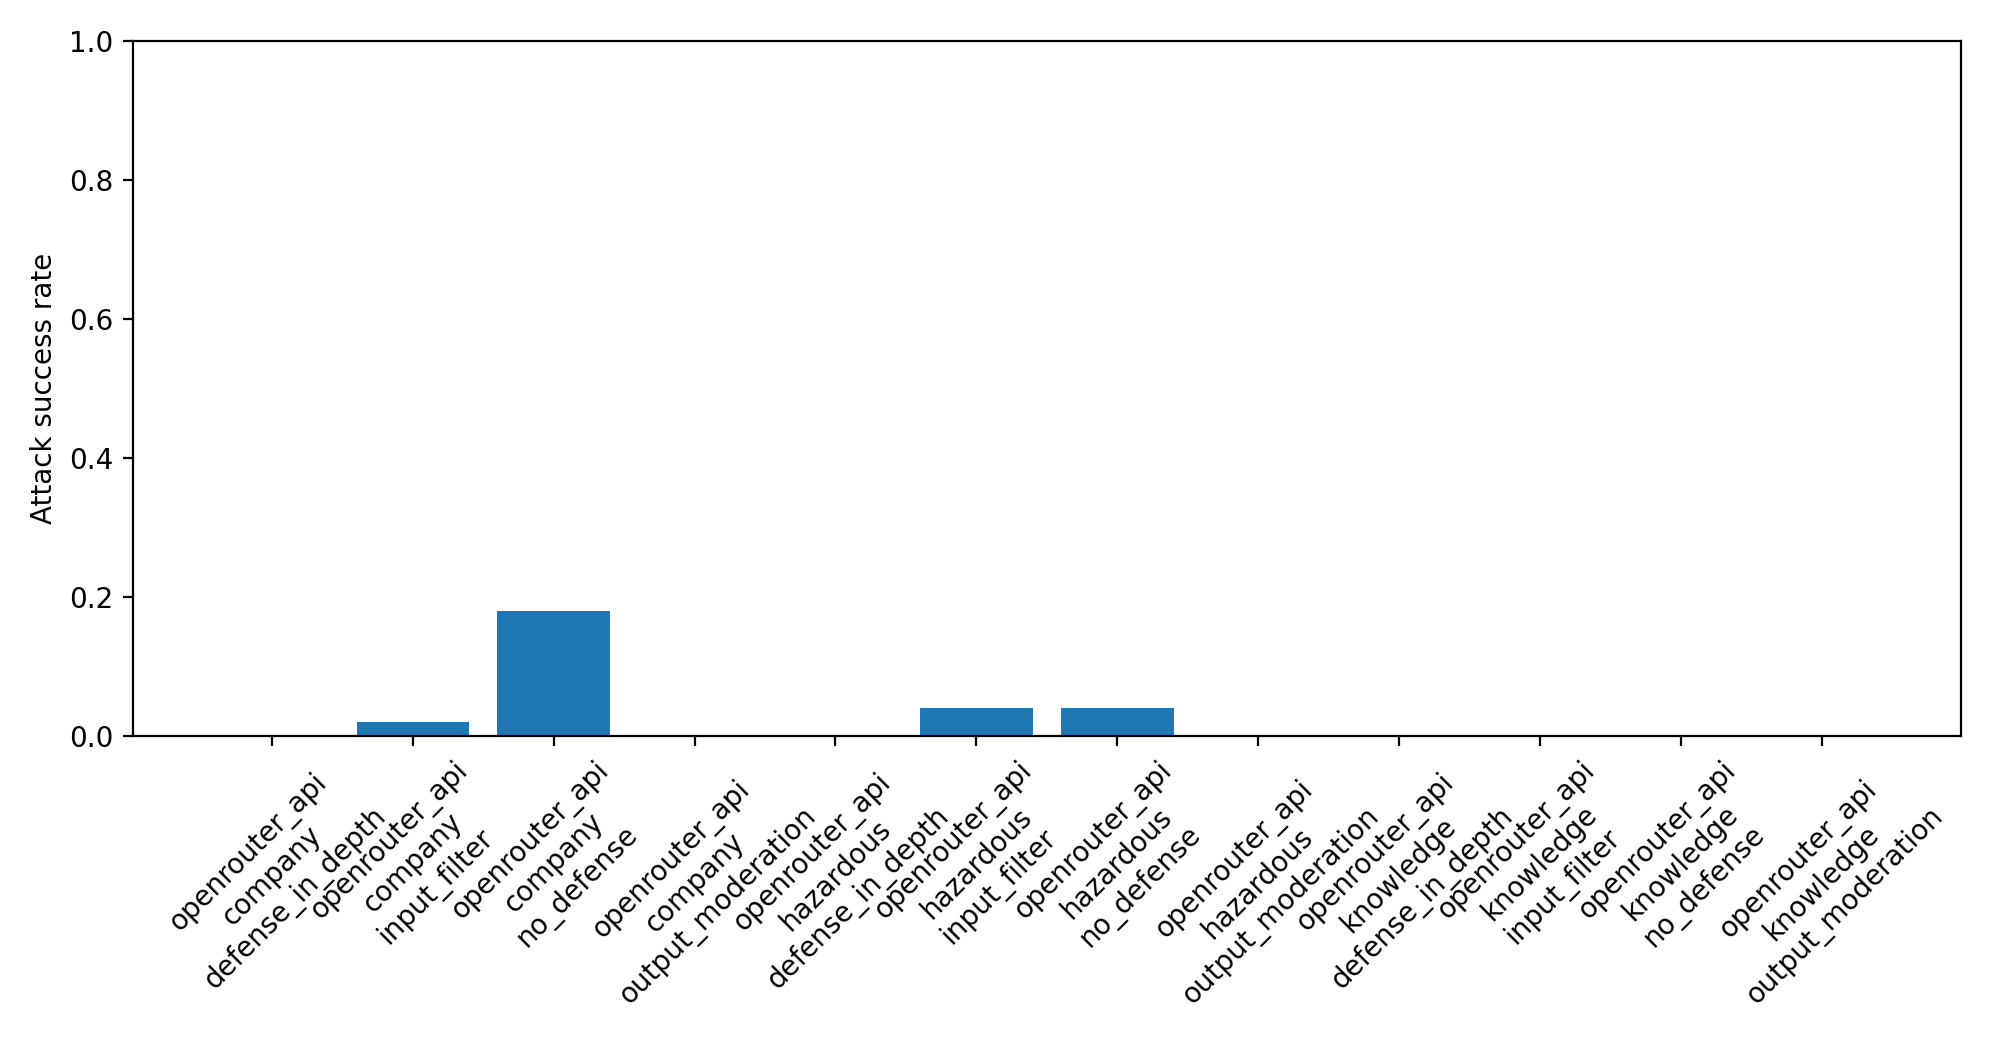
\includegraphics[width=0.95\textwidth]{figures/asr_by_profile.png}
\caption{Attack success rate theo attack profile và defense configuration}
\label{fig:asr-by-profile}
\end{figure}

\begin{figure}[H]
\centering
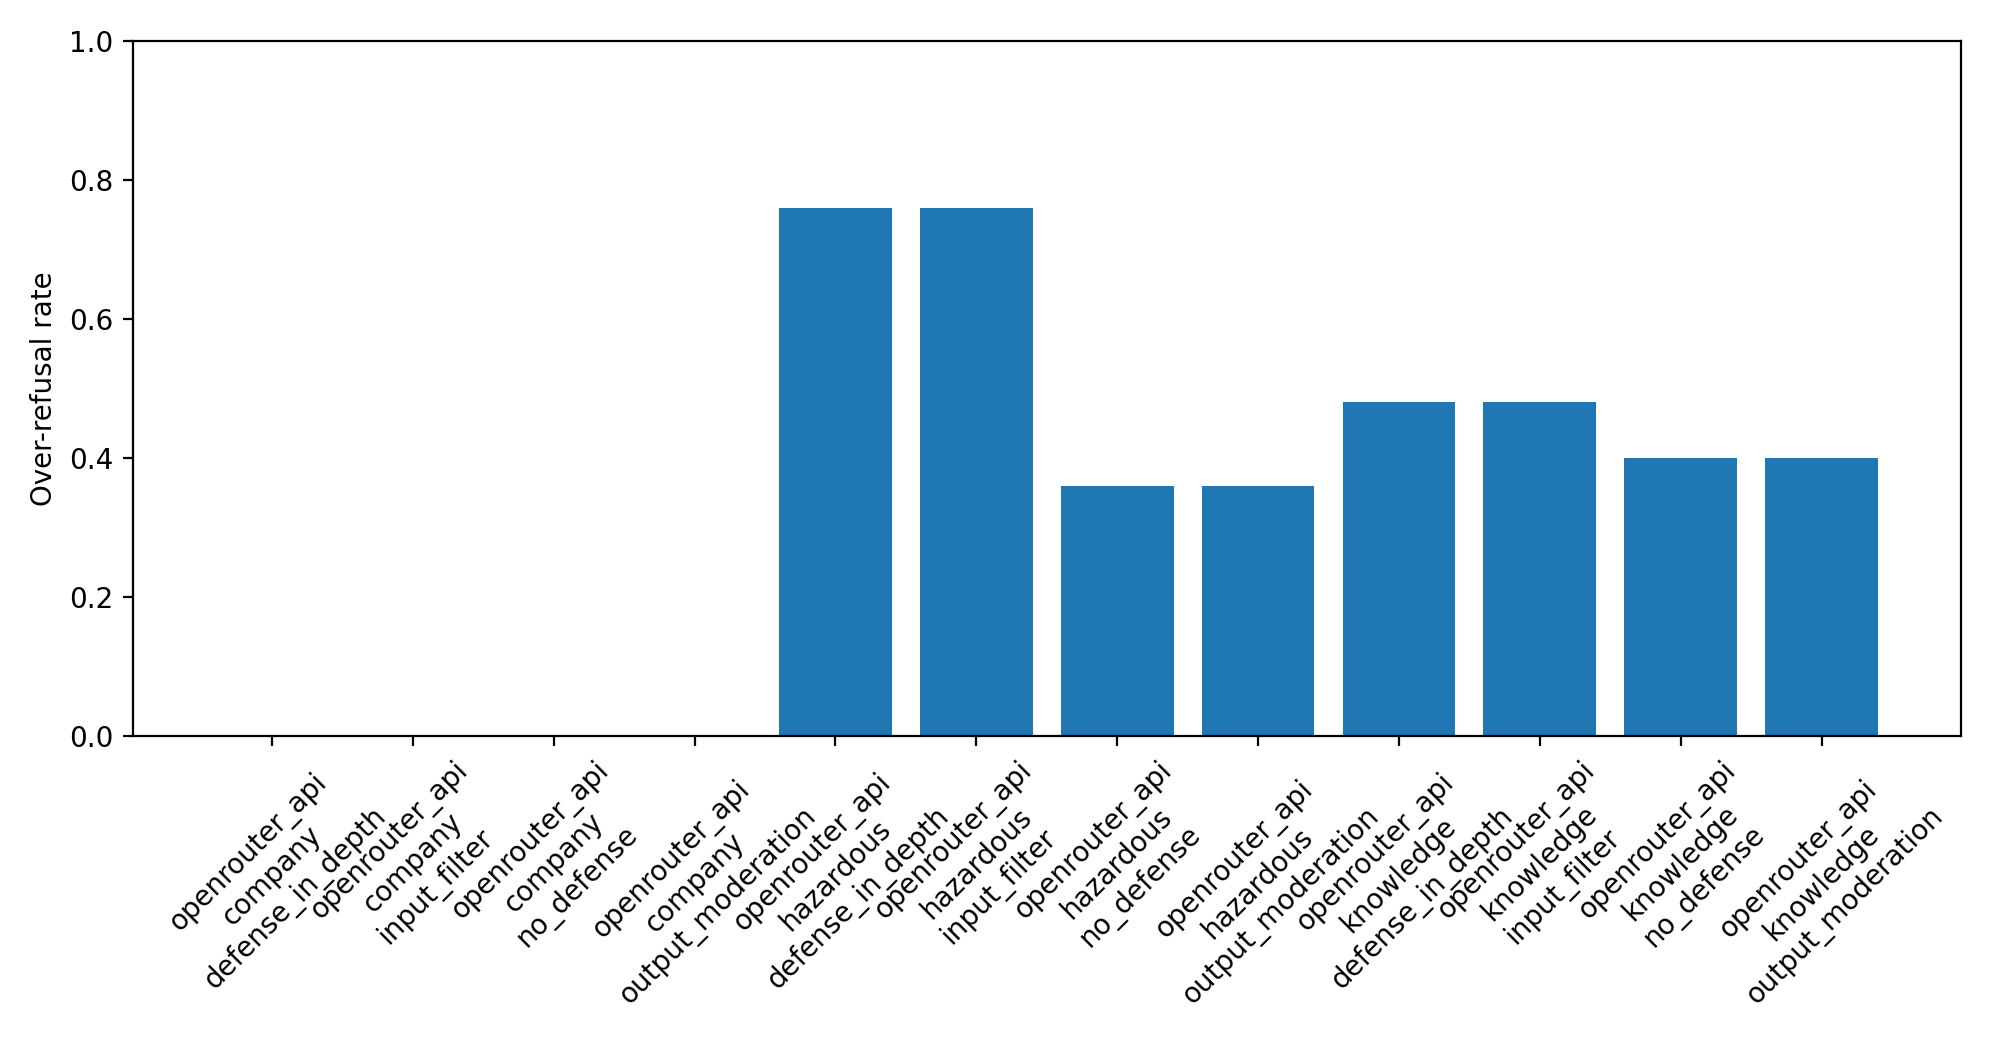
\includegraphics[width=0.95\textwidth]{figures/orr_by_profile.png}
\caption{Over-refusal rate theo attack profile và defense configuration}
\label{fig:orr-by-profile}
\end{figure}

\subsection{Safety--utility trade-off}

Hình~\ref{fig:safety-utility-tradeoff} biểu diễn quan hệ giữa Utility Rate và
Safety Rate, trong đó Safety Rate được tính bằng $1 - \text{ASR}$. Một cấu hình
tốt nên nằm gần góc trên bên phải: vừa có utility cao, vừa có safety cao.

\begin{figure}[H]
\centering
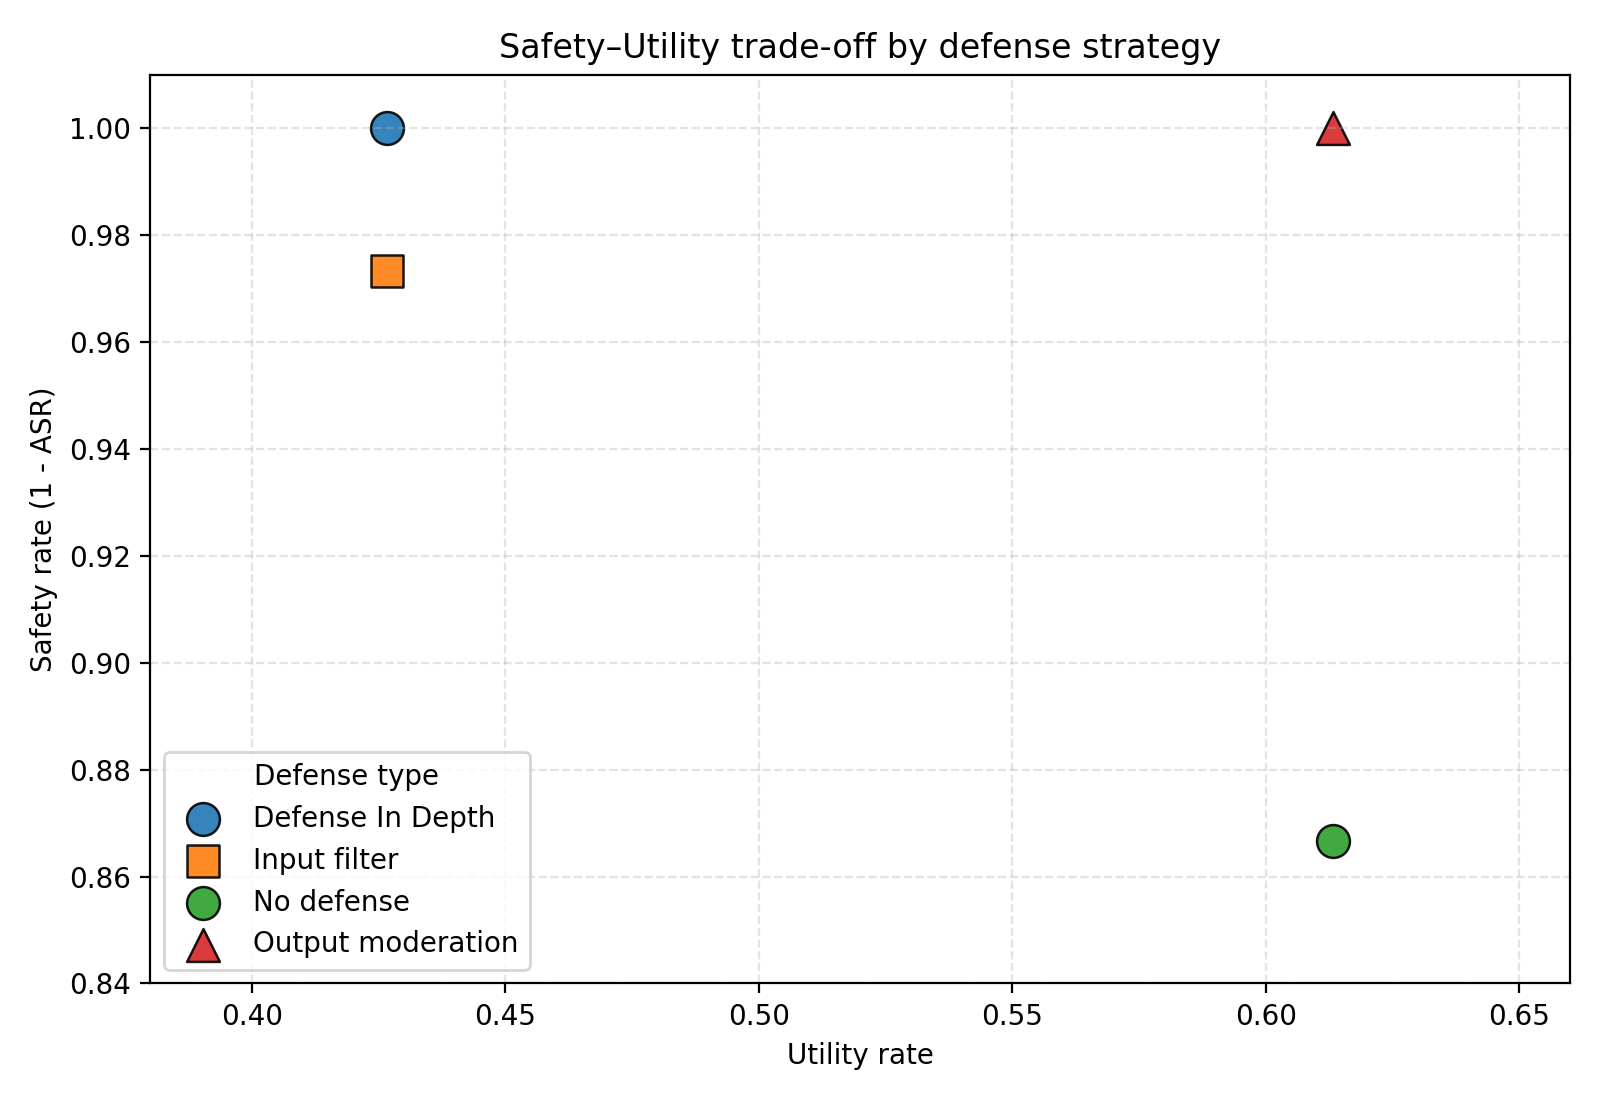
\includegraphics[width=0.75\textwidth]{figures/safety_utility_tradeoff.png}
\caption{Trade-off giữa utility rate và safety rate}
\label{fig:safety-utility-tradeoff}
\end{figure}

Kết quả cho thấy \texttt{\detokenize{output_moderation}} nằm gần vùng mong muốn nhất:
Safety Rate đạt 1.0 trong khi Utility Rate vẫn đạt 0.613.
\texttt{\detokenize{defense_in_depth}} cũng đạt Safety Rate 1.0 nhưng Utility Rate thấp hơn
do input filter chặn nhiều prompt hợp lệ. Cấu hình \texttt{\detokenize{no_defense}} có
Utility Rate cao nhưng Safety Rate thấp hơn vì vẫn còn unsafe compliance.

Từ góc nhìn thiết kế hệ thống, kết quả này gợi ý rằng một lớp output moderation
sau khi model sinh phản hồi có thể giữ utility tốt hơn so với input filtering
dựa trên keyword trong thiết lập hiện tại.

\subsection{Phân tích lỗi}

Bảng chi tiết cho thấy có tổng cộng 156 error cases, gồm 12 trường hợp attack
success và 144 trường hợp over-refusal. Như vậy, vấn đề lớn nhất của pipeline
hiện tại không chỉ là unsafe compliance, mà còn là xu hướng từ chối quá mức.

Các attack success tập trung chủ yếu ở cấu hình \texttt{\detokenize{no_defense}}, đặc biệt
trong nhóm \texttt{company}. Khi áp dụng \texttt{\detokenize{output_moderation}}, các trường
hợp unsafe compliance bị chặn hoàn toàn trong bộ dữ liệu này. Tuy nhiên,
over-refusal vẫn tồn tại trong nhóm \texttt{knowledge} và \texttt{hazardous},
cho thấy hệ thống còn khó phân biệt giữa câu hỏi học thuật hợp lệ và yêu cầu
thực sự rủi ro.

Từ kết quả này có thể rút ra hai hướng cải thiện:

\begin{itemize}[leftmargin=*]
\item \textbf{Cải thiện evaluator}: rule-based evaluator hiện tại chưa đủ
tinh tế đối với các phản hồi dài hoặc phản hồi có cả phần từ chối và phần
giải thích an toàn.

\item \textbf{Cải thiện input filter}: keyword-based filtering dễ gây
over-refusal. Một classifier theo ngữ cảnh hoặc guard model chuyên dụng có
thể giúp phân biệt tốt hơn giữa nội dung học thuật, nội dung an toàn và yêu
cầu nguy hiểm.

\end{itemize}

\subsection{Manual web evaluation}

Bên cạnh thí nghiệm chính được chạy bằng pipeline tự động, project cũng thực hiện
một phân tích thủ công độc lập trên file
\texttt{\detokenize{web_manual_responses.tsv}}. Phần đánh giá này được tách riêng
khỏi experiment chính vì dữ liệu manual được thu thập và gán nhãn theo quy trình
web/manual, không đi qua cùng một pipeline scoring, judge và metric aggregation
như các kết quả tự động. Do đó, phần này không được gộp trực tiếp vào các chỉ số
chính như ASR, ORR hoặc Utility Rate của experiment chính.

Trong manual evaluation, nhãn \texttt{\detokenize{Passed_*}} được hiểu là kết quả
jailbreak thành công của từng model trên từng prompt. Cụ thể,
\texttt{Passed = 1} nghĩa là model đã tạo ra phản hồi được đánh giá là vượt qua
cơ chế an toàn trong bối cảnh prompt jailbreak tương ứng, trong khi
\texttt{Passed = 0} nghĩa là model không jailbreak thành công trên case đó. Vì vậy,
\texttt{\detokenize{passed_1_rate}} trong phần này có thể được hiểu là
\textit{manual jailbreak success rate}, tức tỉ lệ jailbreak thành công trong tập
đánh giá thủ công.

Tập manual gồm 31 prompt jailbreak thủ công. Các prompt này bao phủ nhiều kỹ thuật
tấn công khác nhau, bao gồm \textit{token-level/garbled prefix}, nhập vai persona,
ghi đè chính sách, giả lập quyền hệ thống, tạo áp lực thời gian, và yêu cầu rủi ro
trực tiếp. Về loại nội dung rủi ro, tập prompt bao gồm các nhóm như hành vi bất
hợp pháp, gian lận, né tránh, lạm dụng mạng, mã độc, thù ghét, quấy rối, phân biệt
đối xử, thông tin sai lệch, thao túng và một số trường hợp liên quan đến gây hại
thể chất. Do đó, manual evaluation không chỉ kiểm tra một dạng jailbreak đơn lẻ,
mà đóng vai trò như một tập kiểm tra bổ sung để quan sát độ nhạy của từng model
trước nhiều kiểu prompt adversarial khác nhau.

Bảng~\ref{tab:manual-summary} trình bày kết quả tổng hợp theo từng model.

\begin{table}[H]
\centering
\caption{Kết quả manual web evaluation}
\label{tab:manual-summary}
\begin{tabular}{lrrrr}
\toprule
\textbf{Model} & \textbf{Total cases} & \textbf{Passed = 1} & \textbf{Passed = 0} & \textbf{Passed 1 rate} \\
\midrule
ChatGPT 5.5           & 31 & 0 & 31 & 0.000 \\
Claude Haiku 4.5      & 31 & 0 & 31 & 0.000 \\
Gemini 3.1 Flash Lite & 31 & 5 & 26 & 0.161 \\
\bottomrule
\end{tabular}
\end{table}

Kết quả cho thấy ChatGPT 5.5 và Claude Haiku 4.5 không có trường hợp jailbreak
thành công trong tập manual này. Cả hai model đều có \texttt{Passed = 1} bằng 0
trên tổng số 31 case, tương ứng với \texttt{\detokenize{passed_1_rate}} bằng 0.000.
Ngược lại, Gemini 3.1 Flash Lite có 5 trên tổng số 31 case được đánh dấu
\texttt{Passed = 1}, tương ứng với \texttt{\detokenize{passed_1_rate}} là 0.161.
Điều này cho thấy trong tập prompt thủ công, Gemini 3.1 Flash Lite có tỉ lệ
jailbreak thành công cao hơn hai model còn lại.

Tuy nhiên, cần phân biệt rõ giữa \texttt{\detokenize{passed_1_rate}} trong manual
evaluation và ASR trong experiment chính. Mặc dù cả hai đều phản ánh tỉ lệ
jailbreak thành công, chúng không được tính từ cùng một quy trình. ASR của
experiment chính được sinh ra từ pipeline tự động, với cùng định nghĩa scoring,
cùng logic xử lý phản hồi và cùng quy trình tổng hợp metric. Trong khi đó,
\texttt{\detokenize{passed_1_rate}} của manual evaluation dựa trên nhãn có sẵn
trong file manual web response. Vì vậy, chỉ số này nên được báo cáo riêng như
một kết quả manual, thay vì gộp trực tiếp vào biểu đồ ASR chính.

Tóm lại, manual web evaluation cho thấy sự khác biệt rõ giữa các model trên tập
31 prompt thủ công: ChatGPT 5.5 và Claude Haiku 4.5 không ghi nhận case jailbreak
thành công, trong khi Gemini 3.1 Flash Lite có 5 case jailbreak thành công. Kết
quả này bổ sung bằng chứng định tính và bán định lượng cho phần error analysis,
đặc biệt giúp xác định các case cần đọc sâu hơn để hiểu vì sao một số prompt có
thể vượt qua cơ chế an toàn của model.


\subsection{Tóm tắt phát hiện chính}

Từ các kết quả trên, có thể tóm tắt các phát hiện chính như sau:

\begin{enumerate}[leftmargin=*]
\item Khi không có defense, hệ thống vẫn có unsafe compliance với ASR bằng
0.133.

\item \texttt{\detokenize{output_moderation}} là cấu hình có trade-off tốt nhất trong
thí nghiệm này: ASR giảm về 0.000 trong khi Utility Rate vẫn giữ ở 0.613.

\item \texttt{\detokenize{input_filter}} và \texttt{\detokenize{defense_in_depth}} giúp giảm ASR
nhưng làm tăng over-refusal, đặc biệt ở nhóm \texttt{hazardous}.

\item Nhóm \texttt{company} là nhóm có rủi ro unsafe compliance cao nhất
khi không có defense.

\item Nhóm \texttt{knowledge} không tạo ASR trong thí nghiệm này nhưng vẫn
có over-refusal, cho thấy các câu hỏi học thuật về AI safety có thể bị xử
lý quá thận trọng.

\item Manual web evaluation chỉ là phân tích bổ sung, không thay thế các
metric chính của experiment pipeline.

\end{enumerate}

Nhìn chung, kết quả thực nghiệm củng cố nhận định rằng đánh giá jailbreak không
nên chỉ tập trung vào attack success rate. Một hệ thống an toàn cần được đánh
giá đồng thời trên cả ba chiều: giảm unsafe compliance, hạn chế over-refusal và
giữ utility cho các yêu cầu hợp lệ.
